\section{Bin Width Correction}\label{sec:binCorr}
As shown in Fig.~\ref{reweight}, the distributions of multiplicity skew a lot so that in a certain bin, the center of the bin may not 
represent an ideal horizontal coordinate for plotting the results, especially for the small and large multiplicity regions. 
To study the effect, 10000 fitting trials are done in Monte Carlo. In each trial, in a certain multiplicity region of the three different binning schemes (PVNTRACKS, nForwardTracks, and nBackTracks), 
we randomly sample the mean values of the multiplicity region from a Gaussian sampling, within each bin, mean being the content of the bin and width being the error of the bin. 
Then we fit the 10000 mean values with gaussian distribution to get the central values and uncertainties. To choose a point at which to plot the data, we make the average value of 
the central values we get from the fit. Since the data point is a ratio between two species, \jpsi, and \psitwos, the average value for the ratio is weighted by the inverse of the square of the 
uncertainties (following the PDG weighted average procedure). An example is shown in Fig.~\ref{FitGausMultiplicity}.
\begin{figure}[H]
    \begin{center}
      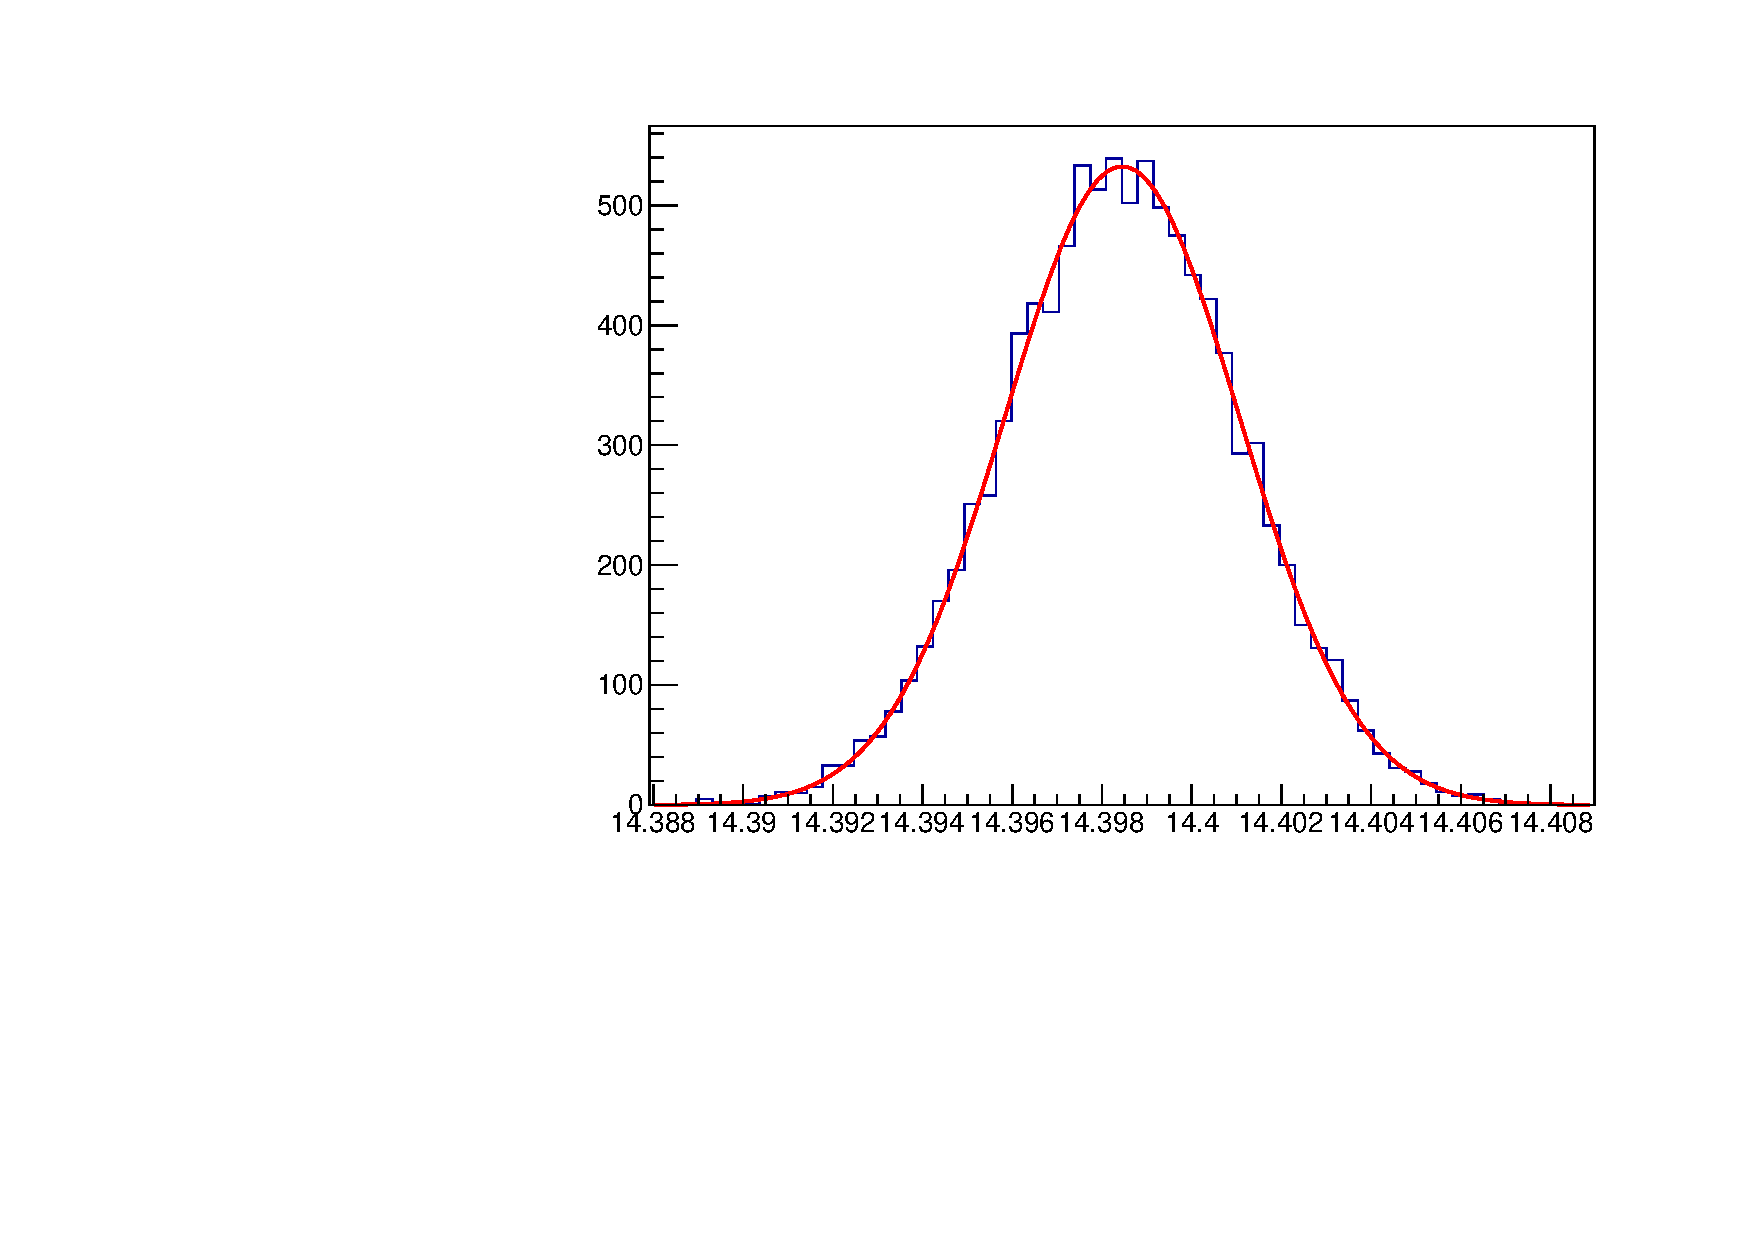
\includegraphics[width=0.3\linewidth]{pdf/Result/JpsiPrompt_0_to_20.pdf}
      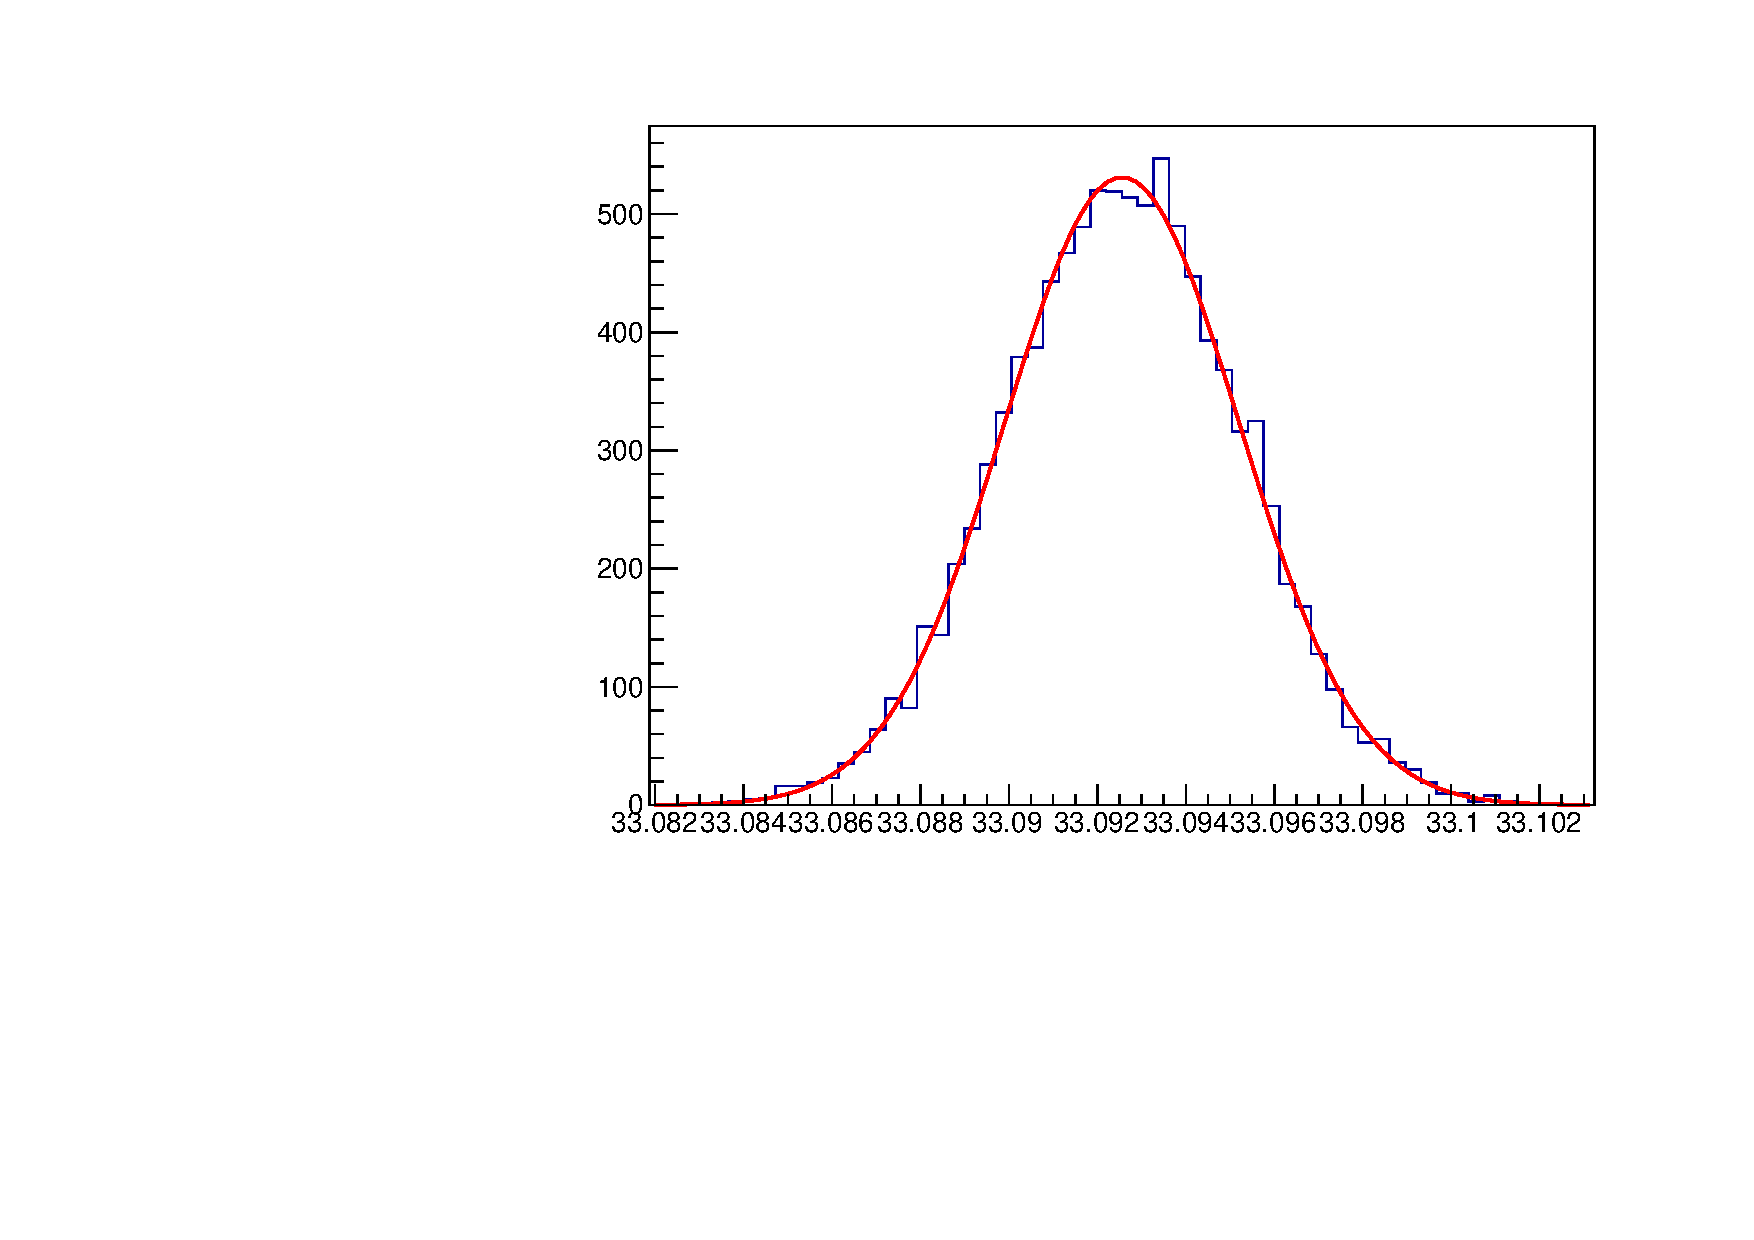
\includegraphics[width=0.3\linewidth]{pdf/Result/JpsiPrompt_20_to_45.pdf}
      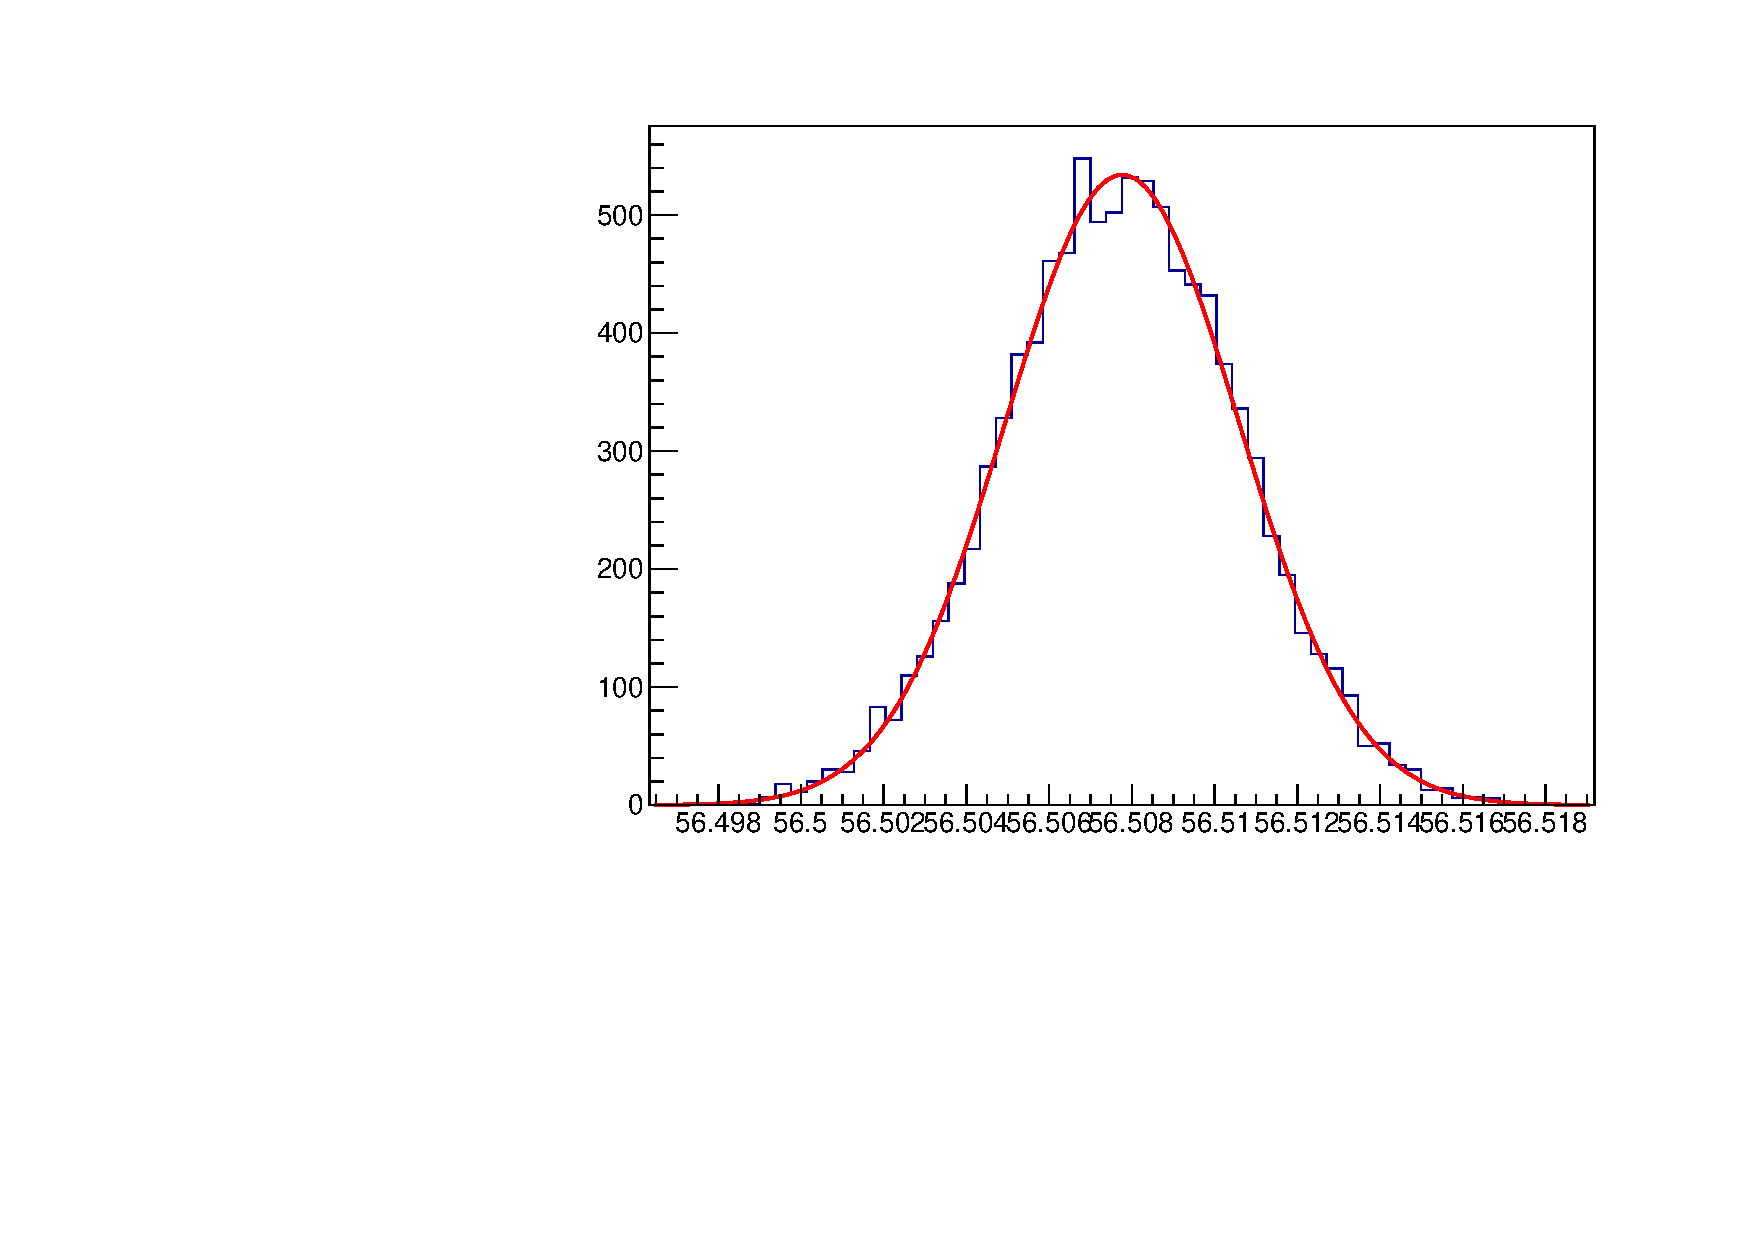
\includegraphics[width=0.3\linewidth]{pdf/Result/JpsiPrompt_45_to_70.pdf}
      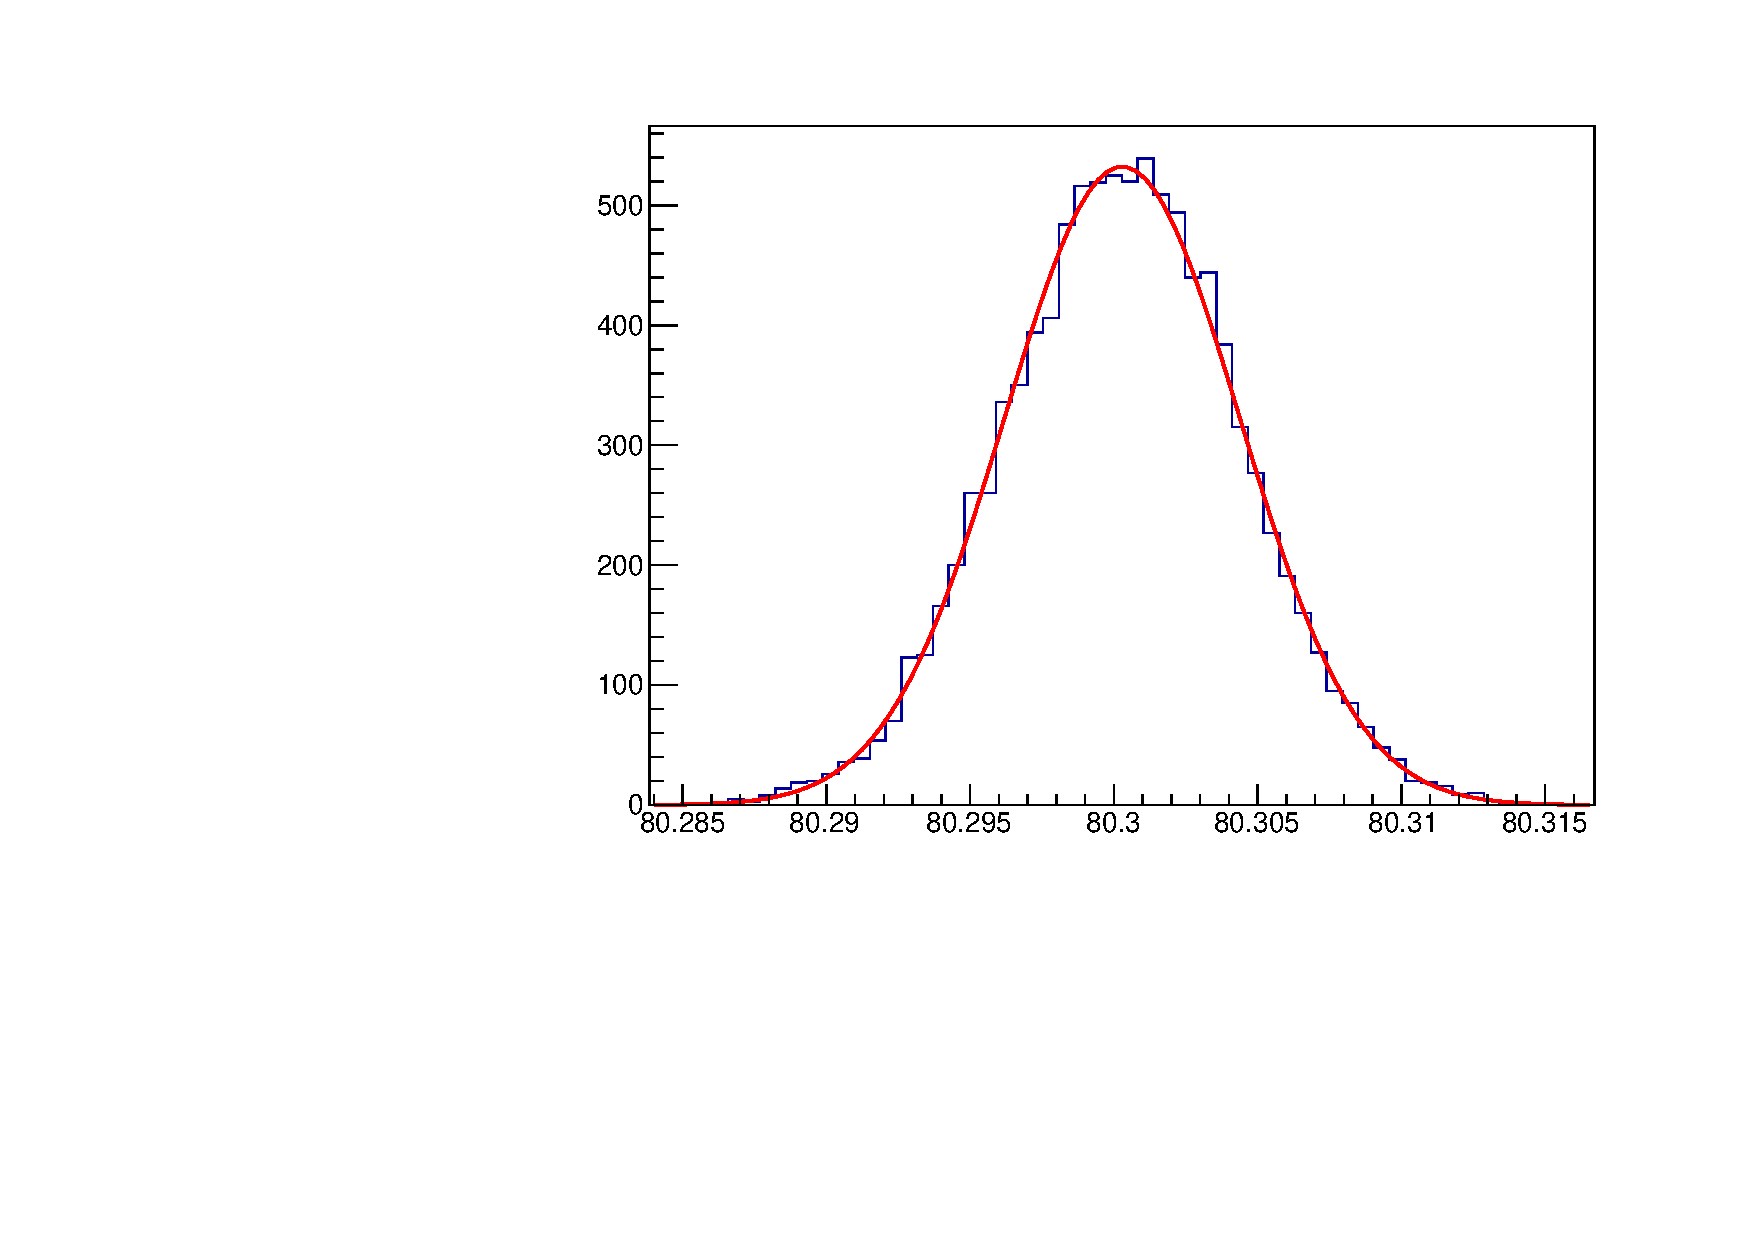
\includegraphics[width=0.3\linewidth]{pdf/Result/JpsiPrompt_70_to_95.pdf}
      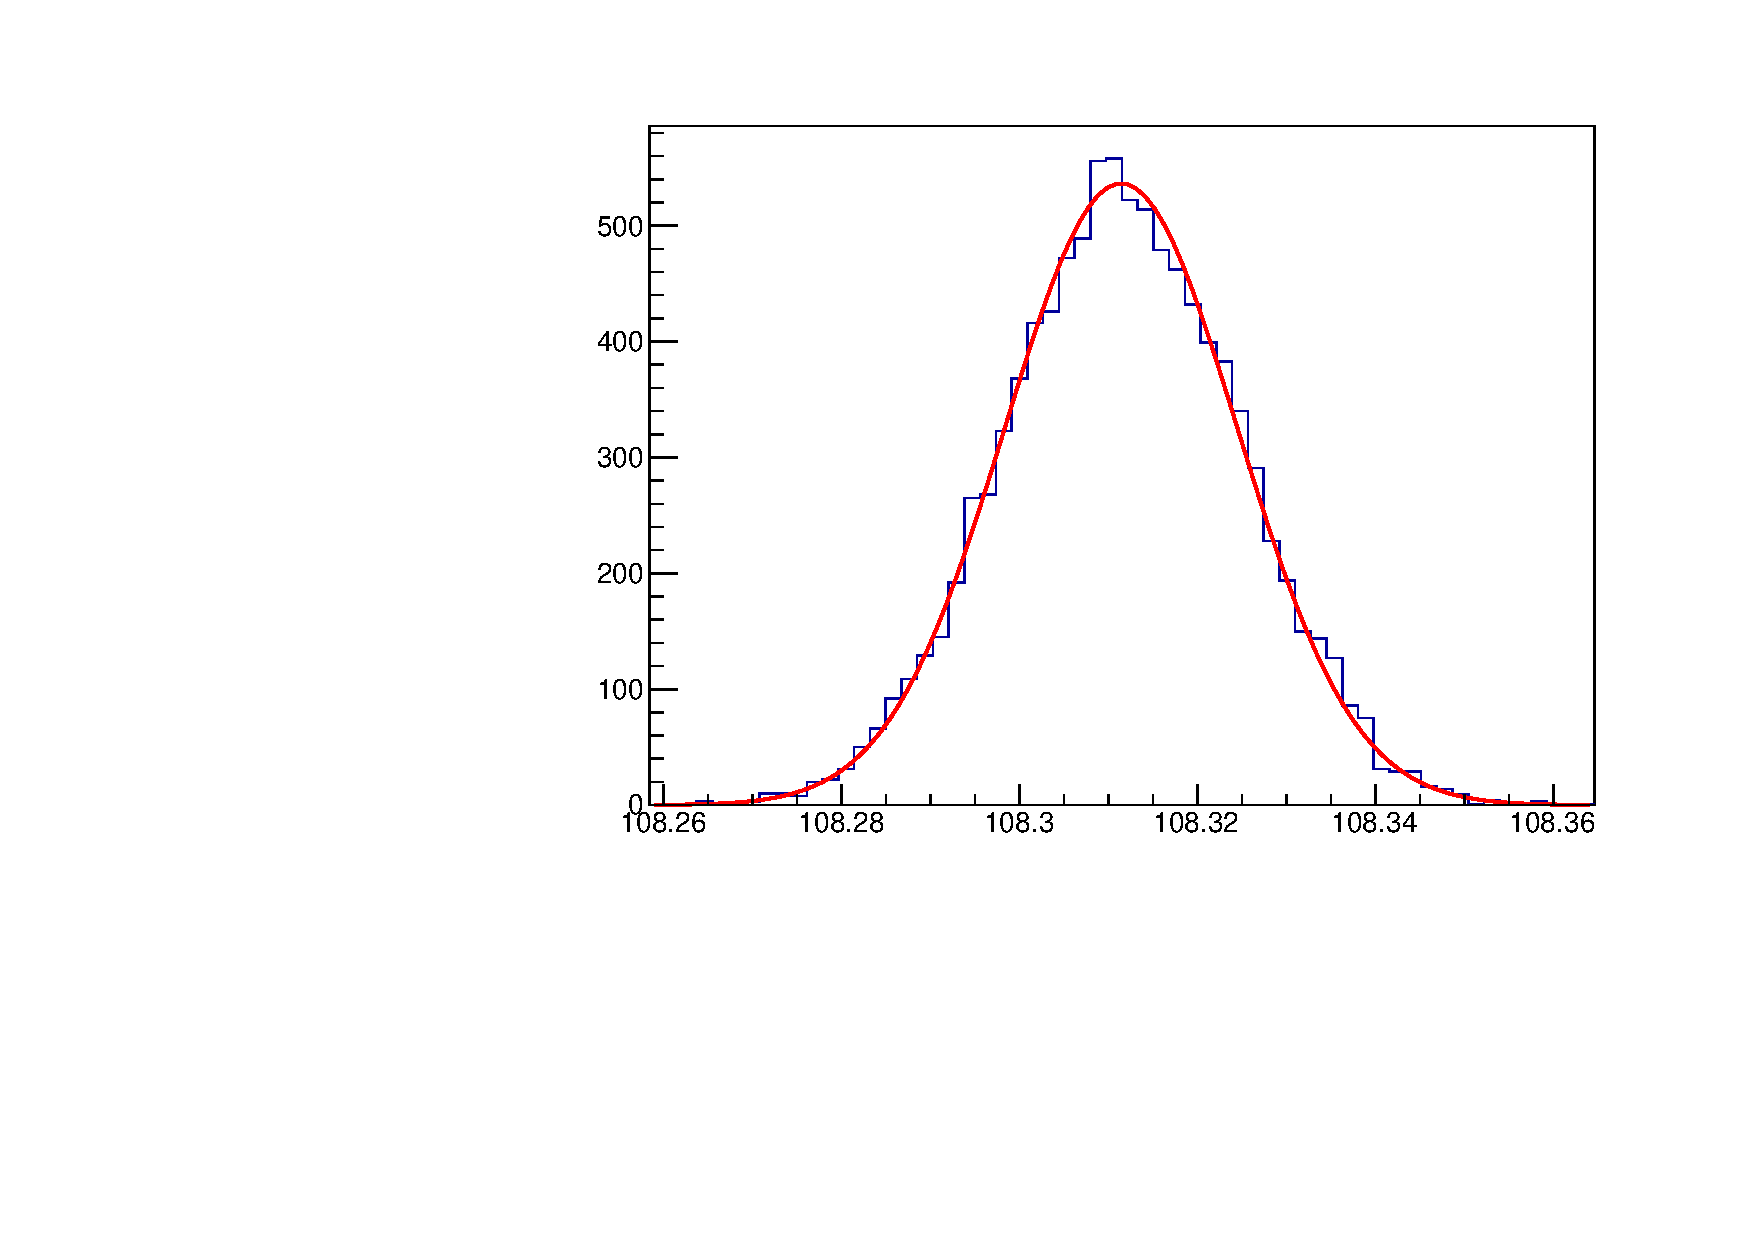
\includegraphics[width=0.3\linewidth]{pdf/Result/JpsiPrompt_95_to_200.pdf}
    \end{center}
	\caption{The distribution of mean value of PVNTRACKS for prompt \jpsi signal in each multiplicity region, which are 4$\leq$ PVNTRACKS$<$20,20$\leq$ PVNTRACKS$<$45,45$\leq$ PVNTRACKS$<$70,70$\leq$ PVNTRACKS$<$95,95$\leq$ PVNTRACKS$<$200. }
  \label{FitGausMultiplicity}
\end{figure}
After finding the proper horizontal coordinates in each multiplicity region, they are further normalized by dividing the mean value of that into no-biased data. 
Finally, the horizontal coordinates for each species are summarized in Table~\ref{XC}.
\begin{table}[H]
  \centering
  \caption{The horizontal coordinates for different binning schemes.}
\begin{center}
  \begin{tabular}{|c|ccccc|}
    \hline
    PVNTRACKS &  4-20 & 20-45  & 45-70   & 70-95   & 95-200   \\ \hline
    prompt & 0.5571 & 1.2791 & 2.1836 & 3.1028 & 4.1852 \\
    \hline
    from $b$ & 0.5758 & 1.2971 & 2.1861 & 3.1010 & 4.1776 \\
    \hline
    nForwardTracks &  0-12 & 12-24  & 24-36   & 36-48   & 48-130 \\ \hline
    prompt & 0.5404 & 1.1143 & 1.8135 & 2.5216 & 3.7005 \\
    \hline
    from $b$ & 0.5415 & 1.1290 & 1.8179 & 2.5229 & 3.6889 \\
    \hline
    nBackTracks &  0-8 & 8-15  & 15-22   & 22-30   & 30-80  \\ \hline
    prompt & 0.4630 & 1.1746 & 1.8747 & 2.6175 & 3.7708 \\
    \hline
    from $b$ & 0.4938 & 1.1793 & 1.8767 & 2.6183 & 3.7710 \\
    \hline
    \end{tabular}
\end{center}
\label{XC}
\end{table}
  
